\documentclass[11pt]{article}
\usepackage{array, booktabs}
\renewcommand{\baselinestretch}{1.2} 
\usepackage{graphicx}
\usepackage{amsmath}
\usepackage{longtable}
\usepackage[table,x11names]{xcolor}
\usepackage{color, soul}  % for higlighting

\addtolength{\topmargin}{-.975in}
\addtolength{\textheight}{1.0in}
\usepackage{float}
\usepackage{subcaption}
\usepackage{xcolor}
\usepackage{multirow}% http://ctan.org/pkg/multirow
\usepackage{hhline}% http://ctan.org/pkg/hhline
\usepackage{cite}
%===== for the quote====
\usepackage{quoting}
\usepackage[T1]{fontenc} % make " straight 
\usepackage{setspace}
\usepackage{lipsum}
\expandafter\def\expandafter\quote\expandafter{\quote\small\singlespacing}
\usepackage[normalem]{ulem}
\usepackage{framed,color}
\usepackage{mdframed}
\usepackage{fancybox} %doublebox
\usepackage{geometry}
 \geometry{
 a4paper,
 total={170mm,256mm},
 left=30mm,
 top=20mm,
 right=30mm,
 }
\begin{document}
\title{Boiling Study for H, H2, H3 and He3 Targets}
\author{Sheren Alsalmi}
\date{}
\maketitle
\section*{Abstract}
When the beam passes through a cryo-target, the local temperature fluctuations could cause a variation in the target density. This density variation is called \emph{Boiling}, and it increases with increasing current. The density fluctuation due to passing beam, or the boiling effect, for jlab Tritium experiments has been studied for Hydrogen (H), Deuterium (H2), Tritium (H3) and Helium (He3) targets.\par
\section{Method Overview}
One way to study the boiling effect is by using the \textbf{Yield Analysis}, where the charge normalized yield is calculated versus current. A decrease in the charged normalized yield at higher currents, indicates that the target's density is decreasing. In another words, the target is \emph{boiling}. \par
\textbf{\underline{Steps for Yield Analysis:}}
\begin{enumerate}
\item{At each current, the total charge is calculated using:
\begin{equation}\label{eq:charge}
Q = a\times \Delta Counts + b\times \Delta Time
\end{equation}
wheren $Q$ is the total charge, $a$ and $b$ are the slop and offset identified by calibrating the Beam Charge Monitors "BCM's" frequency $vs.$ unser current . One can get the $Counts$ and $Time$ from the BCM and Clock scalers respectively. For this study, the dnew BCM is used, and the calibration constants are: $a=0.0003264$ and $b=0.1055$ (see Fig.\ref{fig:dnew})}
\begin{figure}[H]
\centering
 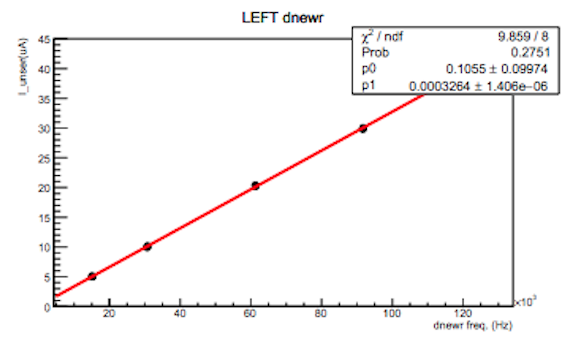
\includegraphics[width=0.7\linewidth]{dnew.png}
  \caption{dnew Calibration by: Nathaly Santiesteban}
  \label{fig:dnew}
\end{figure}
\item{The charge yield of a current $I$, $Yield(I)$, is then calculated using the following:
\begin{equation}\label{eq:y}
Yield(I) = \frac{N_{good}\times PS}{Q\times efficiencies \times LT}
\end{equation}
where $N_{good}$ is the number of good electrons at each current. Determining $N_{good}$,\emph{i.e.} selecting good electrons, is discussed in the following sections. PS and LT are the pre-scale and live-time of each run respectively. The $efficiencies$ include both detectors and trigger efficiencies.}
\item{The charge normalized yield is calculated by normalizing the charge yield for a current $I$, eq.\ref{eq:y}, over the charge yield when there is no current.
\begin{equation}
Y_{norm}(I) = \frac{Yield(I)}{Yield(I=0)}
\end{equation}
Since we don't really know what the charge yield should be at zero current, we use the charge yield at the lowest current available (2.5 $\mu$A for this study) as a normalization factor. Then fit the results so that the normalized yield will be equal to 1 at $I=0$. 

}
\end{enumerate}
\section{Electron Selection:}
  In order to extract a good electron sample, several cuts were applied on the recorded data:
   \begin{enumerate}  
   \item{\textcolor{teal}{\textbf{Selecting Events from Pion Rejector Layers PRL1\&PRL2 and Gas \~Cerenkov GC (PID cut):}}}\par
   To identify the good electrons from the unwanted particles, e.g. pions, only events that leave a pre-specified range of energy on pion rejector layers and Gas \~Cerenkov will be selected .  We refer to this way of Particle IDentification as a \textcolor{purple}{PID cut}. In this analysis, the following PID cuts were applied (see Fig.\ref{fig:prl} \&\ref{fig:cer}):\par
\begin{center}
\framebox(150,85){%
    \parbox{140\unitlength}{L.prl1.e>600 \&\&L.prl2.e>300 \\(L.prl1.e+L.prl2.e)>1700 \\(L.prl1.e+L.prl2.e)<2300 \\L.cer.asum\_c>1000}%
}
\end{center}
\begin{figure}[H]
 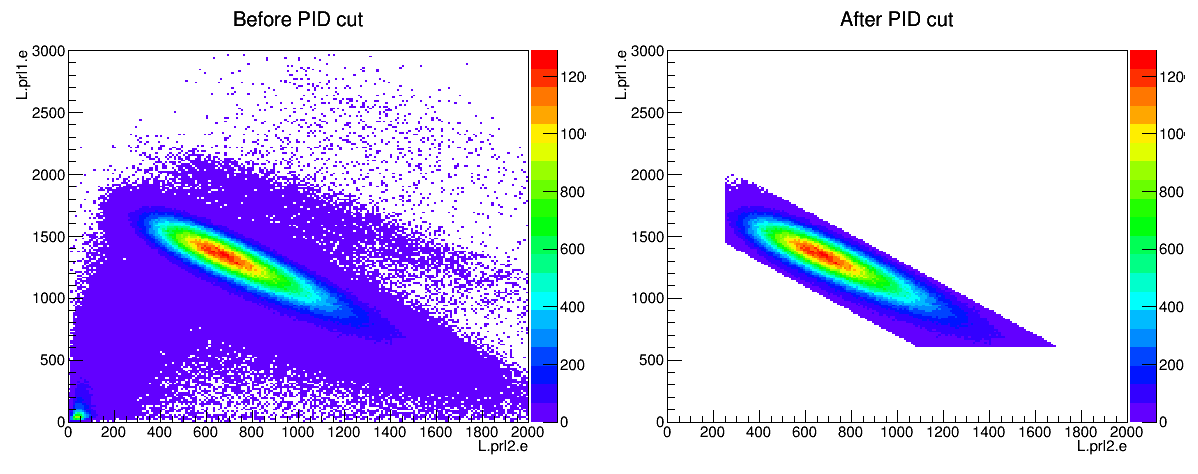
\includegraphics[width=\linewidth]{prl_0.png}
  \caption{PID cut applied on the calorimeters PRL1 \& PRL2 for LHRS}
  \label{fig:prl}
\end{figure}
\begin{figure}[H]
\centering
 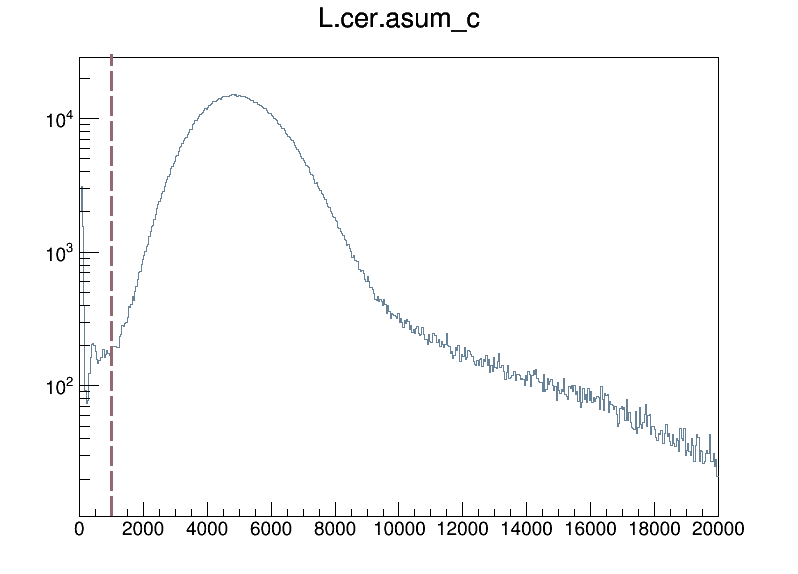
\includegraphics[width=0.6\linewidth]{cer.png}
  \caption{PID cut applied on Gas \~Cerenkov ADC sum}
  \label{fig:cer}
\end{figure}
 \item{\textcolor{teal}{\textbf{Selecting events based on the number of tracks (One-track Cut): }}}\par
 Good events are characterized of leaving only one track on the Vertical Drift Champers VDC. Therefore, only events with one-track were selected, and we call this selection \textcolor{purple}{One-track Cut}
 \begin{center}
\framebox(70,20){%
    \parbox{50\unitlength}{L.tr.n==1}%
}
\end{center}
 \item{\textcolor{teal}{\textbf{Selecting events based on the trigger (Trigger Cut): }}}\par
Three triggers were used during the experiment for LHRS. T1 [S0\&\&S2],  T2 [S0\&\&S2 \&\& GC)] and  T3 [(S0 || S2) \&\& GC)]. T2 is the trigger used through this study. The selection of events that are recorded by a specific trigger is called \textcolor{purple}{Trigger Cut}
  \begin{center}
\framebox(120,20){%
    \parbox{90\unitlength}{DL.evtypebits>>2\&1}%
}
\end{center}
 \item{\textcolor{teal}{\textbf{Selecting events based on the spectrometer acceptance (Acceptance Cut): }}}\par
Electrons that scattered within a specific range of $\theta$, $\phi$ and $\delta$ were selected and let's call this selection the \textcolor{purple}{Acceptance Cuts}. This cut is to make sure that the events are chosen within the acceptance range of the spectrometer. 
 \begin{center}
\framebox(120,60){%
    \parbox{110\unitlength}{abs(L.tr.tg\_th)<0.03\\abs(L.tr.tg\_ph)<0.04\\abs(L.tr.tg\_dp)<0.05}%
}
\end{center}
 \item{\textcolor{teal}{\textbf{Removing events from target end-caps (End-cap Cut): }}}\par
Each cell has two end-caps made of Aluminum. When selecting the good electrons, the events that come from the cell's end-cap need to be excluded. Most of those events can be removed by cutting out the peaks of both end-caps in the $z_{react}$ (or $y_{tar}/sin\theta$) distribution. The following cut on the target length was applied (See Fig.\ref{fig:ycut}):\par
 \begin{center}
\framebox(155,20){%
    \parbox{150\unitlength}{abs(L.tr.tg\_y/$sin\theta$)<0.075 m}%
}
\end{center}
 \begin{figure}[H]
 \centering
 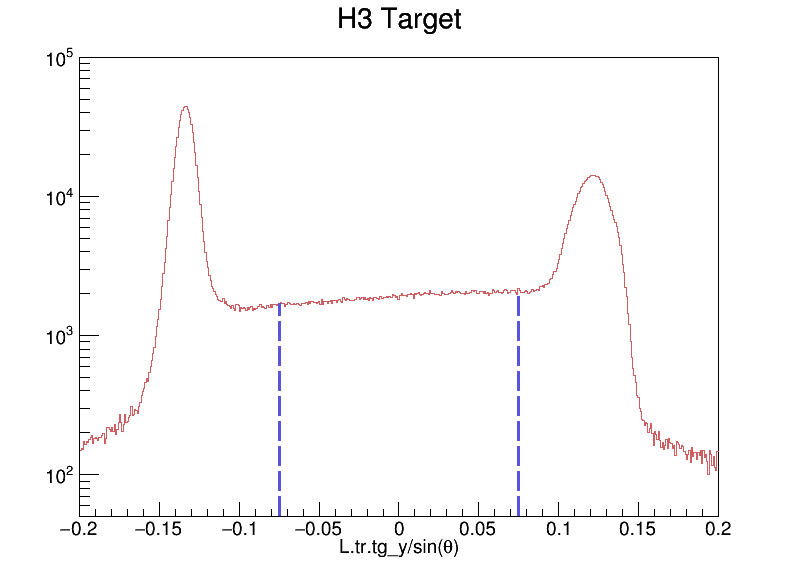
\includegraphics[width=0.6\linewidth]{y_cut.png}
  \caption{Cutting on the target length to git rid of end-cap events}
  \label{fig:ycut}
\end{figure}
However, cutting the end-cap peaks will not remove all of the end-cap events. There are still some Aluminum events mixed with the events from the cryo-target. These end-cap events are called "end-cap background". In order to estimate this background, the following steps were taken:
\clearpage
\begin{itemize}
\item{\underline{Estimating the end-cap background $vs.$ current:}  \par
 In order to check how end-cap background changes with increasing current, a comparison between the background at low and high current was estimated for an empty cell (Fig.\ref{fig:bk_empty}). Each run was normalized over the total charge yield, and the ratio of the events at high current to low current was estimated. The ratio was found to be $\sim$ 1.006, which indicates that the end-cap background will $not$ increase with increasing current and it is a constant number. Therefore, for the charge normalized yield this value will cancel out. However, when calculating the total charge yield, the background events need to be extracted from cryo-target events.}
 \begin{figure}[H]
 \centering
 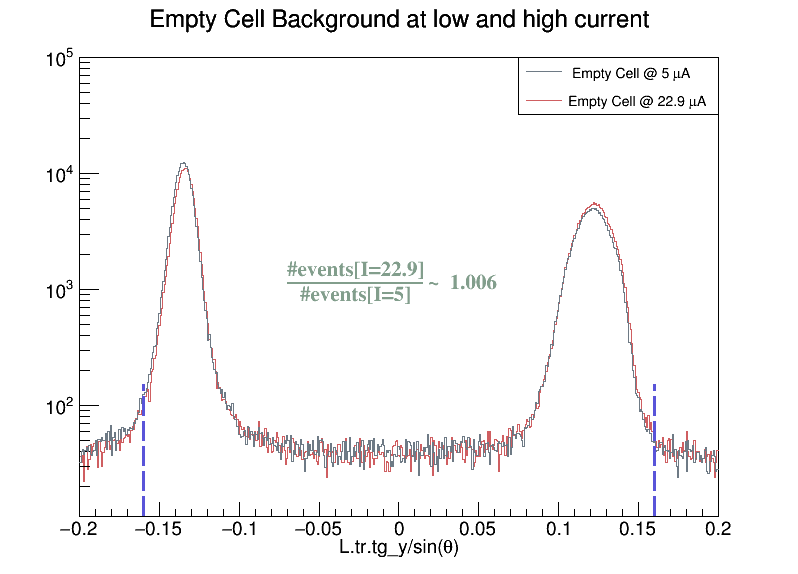
\includegraphics[width=0.6\linewidth]{bk_empty.png}
  \caption{Ratio of end-cap background at high current to low current}
  \label{fig:bk_empty}
\end{figure}
 \item{\underline{Estimating the end-cap background for each cryo-target:}\par
Even though the end-cap background should be the same for low and high current, this background value might be different for each target. To check that, an empty cell run at low current ($\sim$ 5 $\mu$A) was compared to each cryo-target at the same current. Since the windows thickness is different slightly from cell to cell, normalizing over the charge yield did not seem accurate. Calculating the charge yield of two cells by applying same cut on the target length, does not mean necessarily that we picked the same thickness of both windows. We might end up normalizing over the charge yield that came out of two different target thickness. To avoid that, and knowing that the peak at the cell window is proportional to the window's thickness, the upstream windows were scaled to match each other. The two runs, $i.e.$ the empty cell run and the cryo-target run, were normalized so that the maximum number of events at the upstream windows are the same for both runs. To determine the maximum number of events, a gaussian fit about 1 $\sigma$ was made at the peak (see Fig.\ref{fig:scale}). The y-value at the mean of the fit is considered the maximum number of events for that window. Then, the two windows were normalized so that the peak will match. 
\begin{figure}[H]
\centering
\begin{subfigure}{.4\textwidth}
\centering
 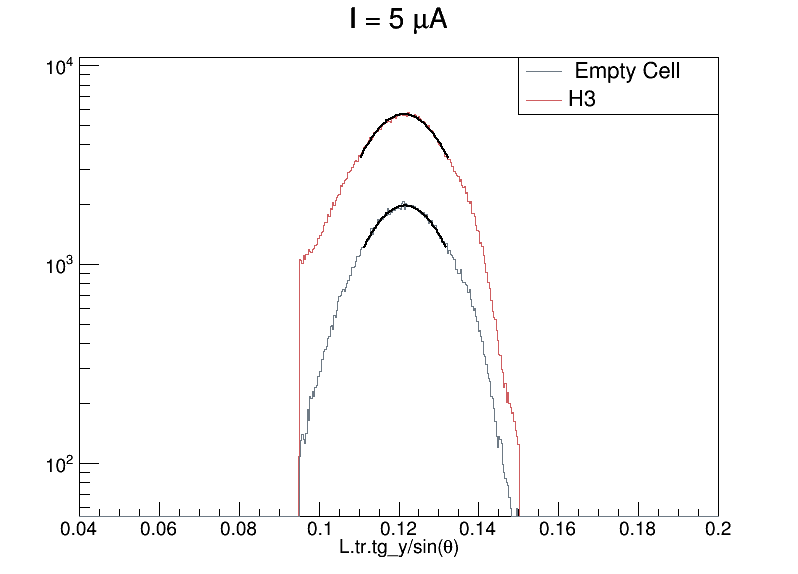
\includegraphics[width=\linewidth]{scale5_H3.png}
  \caption{before normalizing}
  \label{fig:scale1}
\end{subfigure}
\begin{subfigure}{.4\textwidth}
 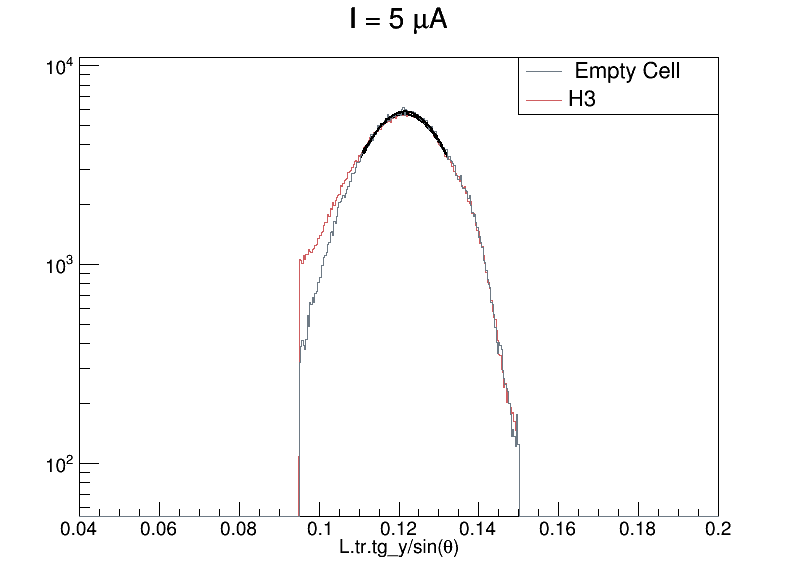
\includegraphics[width=\linewidth]{scale5_H3_2.png}
  \caption{after normalizing}
  \label{fig:scale2}
\end{subfigure}
\caption{Normalizing the upstream window for two runs}
\label{fig:scale}
\end{figure}
After normalizing the upstream windows, the end-cap contamination was calculated as:
\begin{center}
End-cap Contamination = $\frac{\# \text{of good events come from empty cell from -0.075 to 0.075}}{\# \text{of good events come from cryo-cell from -0.075 to 0.075}}$
\end{center}
This way, one can know how many events coming from end-caps \emph{and} that will trick us to be as good electrons. That is the number that will affect the cryo-target charge yield directly. The other events coming from the end-caps, will be cut out with the good electrons cut and shouldn't be extracted from the number of good events used to measure the charge yield. \par
The above method was made for H3, He3, D2 and H and the results are shown in Fig.\ref{fig:endcap}

\begin{figure}[H]
\centering
\begin{subfigure}{.4\textwidth}
\centering
 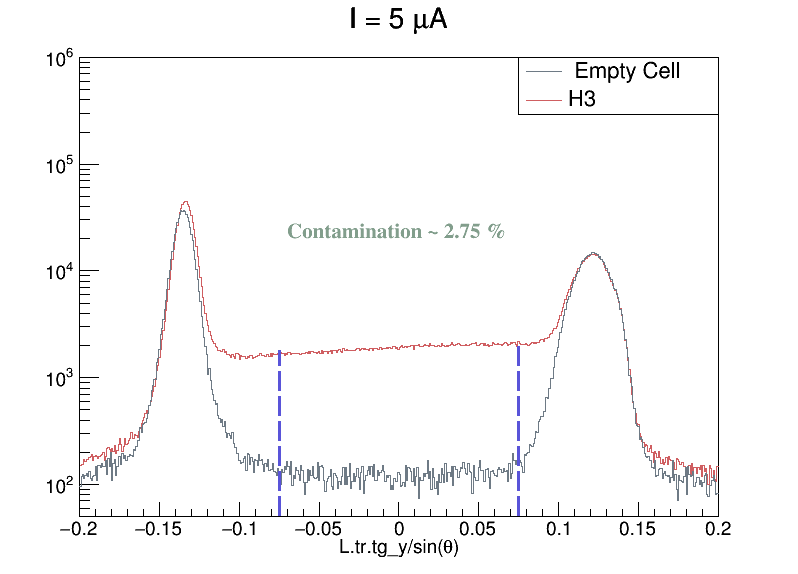
\includegraphics[width=\linewidth]{bk5_H3.png}
  \caption{H3}
\end{subfigure}
\begin{subfigure}{.4\textwidth}
 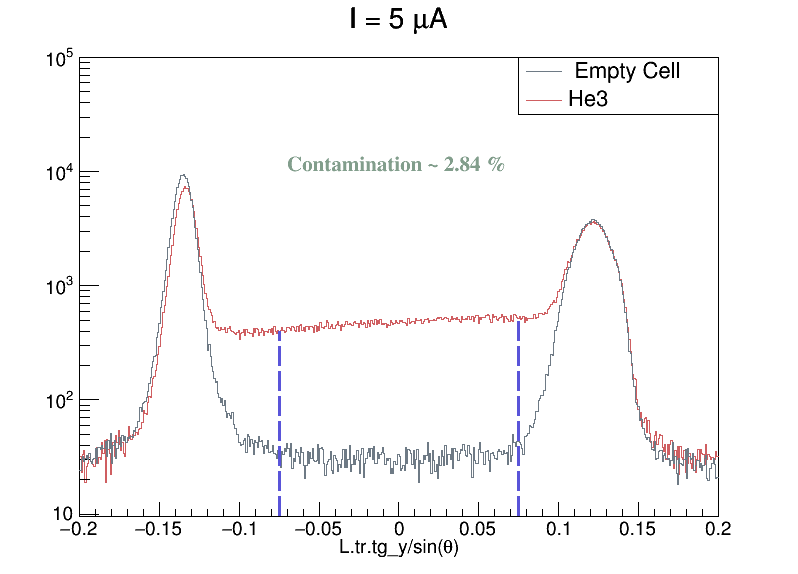
\includegraphics[width=\linewidth]{bk5_He3.png}
  \caption{He3}
\end{subfigure}
\begin{subfigure}{.4\textwidth}
\centering
 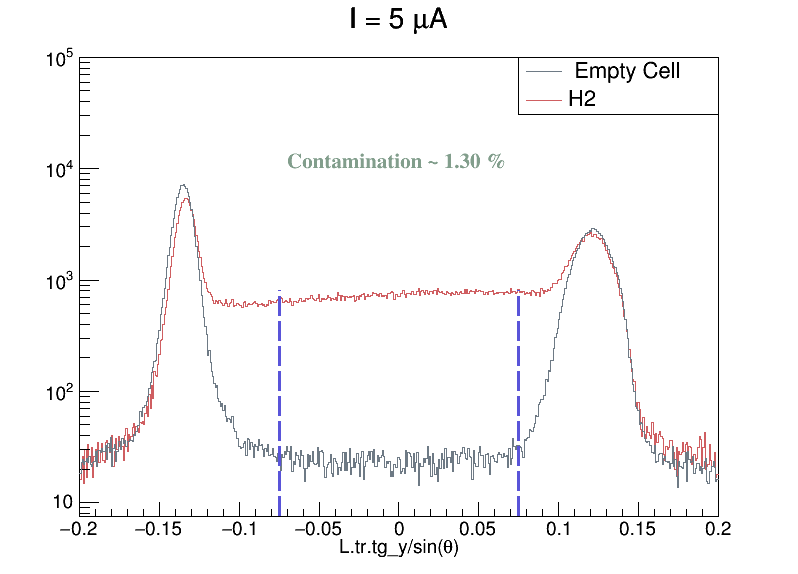
\includegraphics[width=\linewidth]{bk5_H2.png}
  \caption{H2}
\end{subfigure}
\begin{subfigure}{.4\textwidth}
 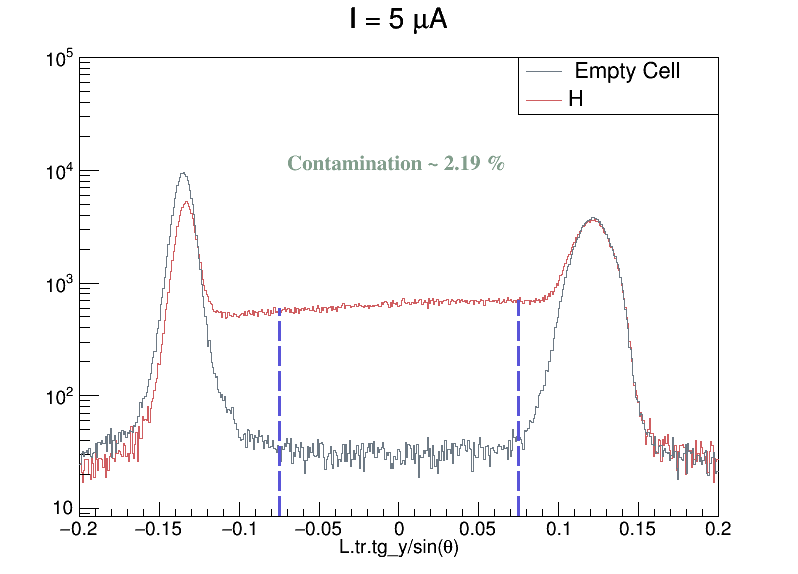
\includegraphics[width=\linewidth]{bk5_H.png}
  \caption{H}
\end{subfigure}
\caption{End-cap Background for each target }
\label{fig:endcap}
\end{figure}
}
When calculating the total charge yield, the end-cap background should be extracted from the total number of good events of each target. However, since this background is assumed to be almost the same with increasing current, the \emph{Normalized} charge yield -which is the main goal of this study- will be the same, i.e. the background will cancel out. The number of charge yield before and after extracting end-cap background will be listed for each target.
\end{itemize}
 \item{\textcolor{teal}{\textbf{Selecting events from a stable beam (Beam Trip Cut): }}}\par
If the beam is stable during the run (see Fig.\ref{fig:stable}), the total charge can calculated using Eq.\ref{eq:charge}. Both $\Delta Counts$ and $\Delta Time$ can be extracted from the scalers at the beginning and the end of the run. If the beam tripped for a small period of time, $i.e.$ at the beginning or end of the run, one can just cut those periods of the run when the beam was tripping, and handle only the period of the run when the beam was stable. However, sometimes the beam trips significantly from time to time during the run (see Fig.\ref{fig:909}), which makes selecting a period of the run with a stable beam hard and maybe not accurate.  It is crucial when selecting the good electrons to make sure that those electrons survived the beam tripping, and we call this selection \textcolor{purple}{Beam Trip Cut} . 
\begin{figure}[H]
\centering
\begin{subfigure}{.4\textwidth}
\centering
 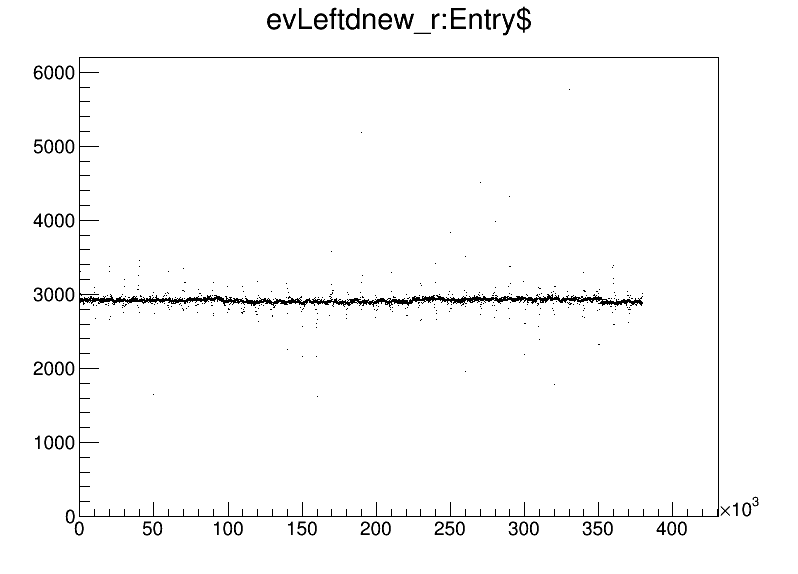
\includegraphics[width=\linewidth]{stable.png}
  \caption{Stable beam}
  \label{fig:stable}
\end{subfigure}
\begin{subfigure}{.4\textwidth}
 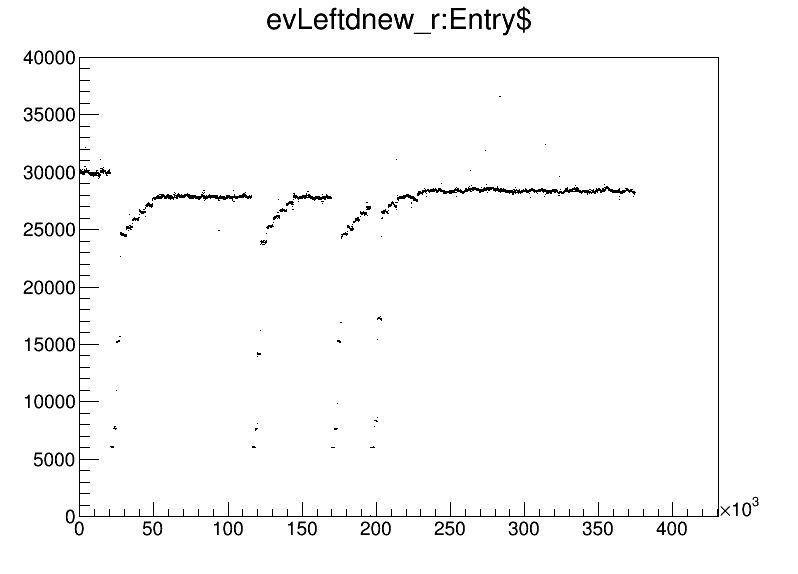
\includegraphics[width=\linewidth]{909.png}
  \caption{Tripping beam}
  \label{fig:909}
\end{subfigure}
\caption{Examples for runs with stable beam and tripping beam}
\label{fig:beam}
\end{figure}
In this analysis, event-by-event check was applied. If the event passed all of the above cuts, $i.e.$ PID, trigger, one track, end-cap and acceptance cuts, then the current that produced that event will be checked. If the current was within $\pm$2$\mu$A  about the current requested for the run, that event will be considered as a \emph{good electron}. Otherwise, the event will be neglected. Fig.\ref{fig:beam} illustrates how the beam trip cut was applied for this study.

%\begin{figure}[H]
%\centering
% \includegraphics[width=0.6\linewidth]{Slide1.jpg}
%  \caption{Applying beam trip cut }
%  \label{fig:beam}
%\end{figure}
%\end{enumerate}
%\section{Efficiencies:}
%\begin{enumerate}
% \item{\textcolor{teal}{\textbf{Gas \~Cerenkov Efficiency ($\epsilon_{cer}$):}}}\par
 
\begin{equation}
\epsilon_{cer}=\frac{N_{e}^{GC}}{N_{e}^{sample}}
\end{equation}
   where $N_{e}^{sample}$ is the number of electrons obtained after applying PRL, trigger, one-track, end-cap, beam trip acceptance cuts to get good electron sample. $N_{e}^{GC}$ is the number of electrons obtained after applying  a \~Cerenkov cut in addition to the same cuts applied to obtain  $N_{e}^{sample}$. 
\item{\textcolor{teal}{\textbf{VDC Efficiency ($\epsilon_{trk=1}$): }}}\par
 The efficiency of the VDC can be obtained by checking the efficiency of the one-track cut as follows: 
\begin{equation}
\epsilon_{trk=1}=\frac{N_{track=1}}{N_{\text{all tracks}}}
\end{equation}
where  $N_{\text{all tracks}}$ is the number of electrons that passes PID (Cer and PRL's) , trigger, end-cap, acceptance and beam trip cuts, that left any track on the VDC's including zero tracks. $N_{track=1}$ is the number of electrons that passed all previous cuts \emph{but} left only one track on the VDC's.
\item{\textcolor{teal}{\textbf{Trigger Efficiency ($\epsilon_{trig}$):}}}\par
As mensioned above, T2 was used to select electrons in this study, and T1 was used to check T2 efficiency as following:
 \begin{equation}
 \epsilon_{trig}=\frac{PS_{T_{2}}\times N_{T_{2}}}{PS_{T_{1}} \times N_{T_{1}}}
  \end{equation}
 where $PS_{T_{i}}$ and $N_{T_{i}}$ are the pre-scale and number of events recorded for trigger type $i$ respectively. The events selected here must pass the PID, one-track, end-cap, acceptance and beam trip cuts. 
  \end{enumerate}
\section{Solid Target Boiling "Check":}
Since the solid target does not change its density with increasing current, the normalized yield should be \~ 1 for any solid target. The upstream and downstream windows of the Tritium cell were selected for this test. The results are shown in Fig.\ref{fig:upstream}
\begin{figure}[H]
  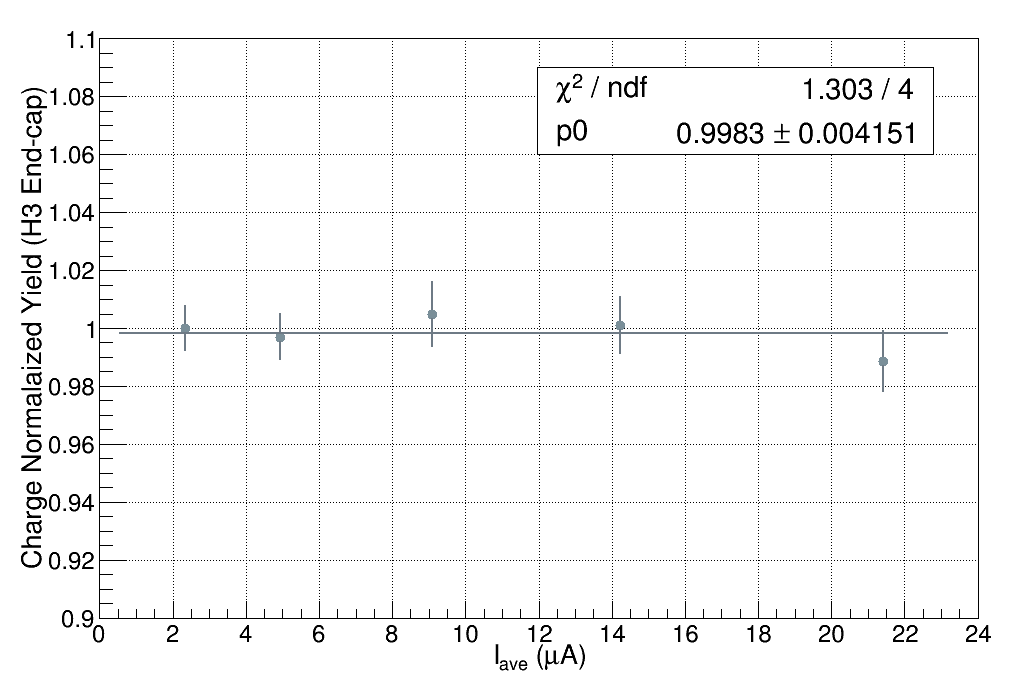
\includegraphics[width=\linewidth]{upstream.png}
  \caption{Charge Normalized Yield for Solid Target (Upstream End-cap of H3 cell)}
  \label{fig:upstream}
\end{figure}
\begin{figure}[H]
  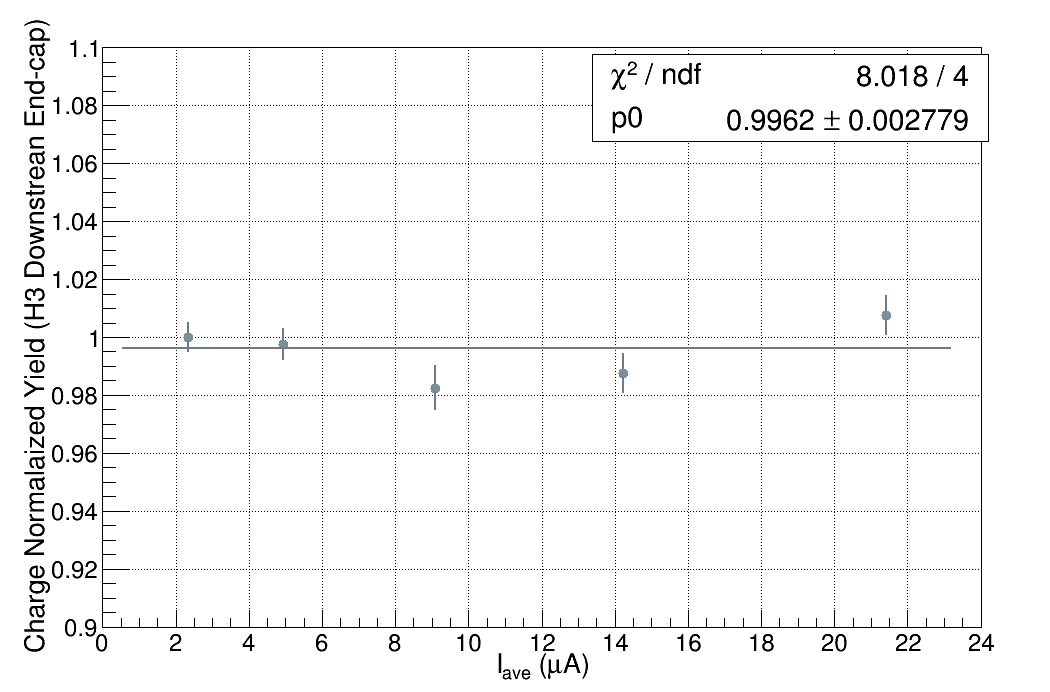
\includegraphics[width=\linewidth]{downstream.png}
  \caption{Charge Normalized Yield for Solid Target (Downstream End-cap of H3 cell)}
  \label{fig:downstream}
\end{figure}

\section{Tritium Target Boiling:}

\begin{table}[H]
\caption{Efficiencies for H3 boiling runs}
\begin{tabular}{|>{\centering}m{0.6in} |>{\centering}m{1.3in}| >{\centering}m{1.3in}| >{\centering}m{1.3in}| >{\centering\arraybackslash}m{1.1in}|}
\hline
 \rowcolor{lightgray} Run & Cerenkov eff. (\%) & one track eff. (\%)  & trigger [T2] eff (\%)& DT (\%) \\
 \hline
902&99.9828&98.6125&98.9123&4.36\\
905&99.9879&98.4400&99.4147&4.43\\
9091&99.9845&98.2996&100.5&2.91\\
910&99.9925&98.0794&100.&4.54\\
911&99.9916&97.8293&99.8825&3.43\\
\hline
\end{tabular} 
\end{table}


\begin{table}[H]
\caption{Normalized Yield H3 Target}
\begin{tabular}{|>{\centering}m{0.3in} | >{\centering}m{0.7in}|>{\centering}m{0.7in}|>{\centering}m{0.7in}| >{\centering}m{0.7in}| >{\centering}m{1in}| >{\centering\arraybackslash}m{0.7in}|}
\hline
 \rowcolor{lightgray} Run & Current ($\mu$A) & \#good events & Total Charge ($\mu$C) &Yield & Charge Normalized Yield&  error \\
 \hline
902&2.343&67998&1964.302&111.350&0.983&0.002\\
905&4.809&64243&4382.545&109.720&0.968&0.002\\
909&9.094&31366&6141.763&106.410&0.939&0.003\\
910&14.232&39032&8009.334&104.013&0.918&0.002\\
911&21.407&34709&14567.098&101.008&0.891&0.003\\
\hline
\end{tabular} 
\end{table}
\begin{figure}[H]
  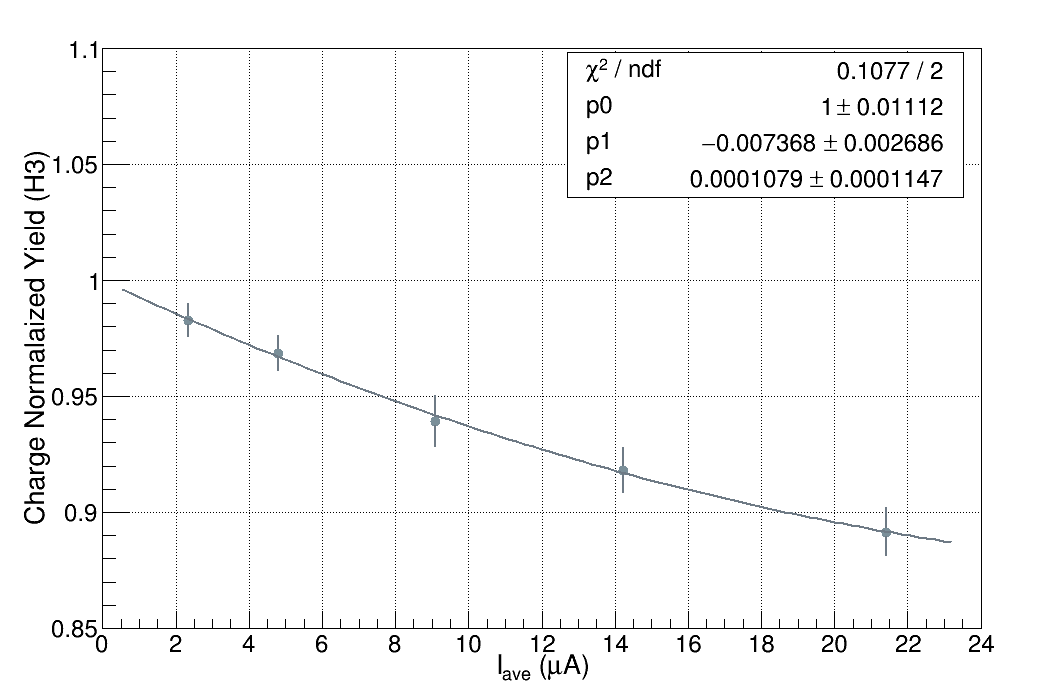
\includegraphics[width=\linewidth]{y_H3_2.png}
  \caption{Charge Normalized Yield for Tritium}
  \label{fig:yT}
\end{figure}

\section{Helium-3 Target Boiling:} 
\begin{table}[H]
\caption{Efficiencies for He3 boiling runs}
\begin{tabular}{|>{\centering}m{0.6in} |>{\centering}m{1.3in}| >{\centering}m{1.3in}| >{\centering}m{1.3in}| >{\centering\arraybackslash}m{1.1in}|}
\hline
 \rowcolor{lightgray} Run & Cerenkov eff. (\%) & one track eff. (\%)  & trigger [T2] eff (\%)& DT (\%) \\
 \hline
916&99.9812&98.7991&100.&3.70\\
915&99.9827&98.7315&101.5&3.14\\
914&99.9927&98.5244&102.2&3.82\\
913&99.9907&98.3497&101.34&3.93\\
912&99.9851&98.0509&102.7&2.83\\
\hline
\end{tabular} 
\end{table}
\begin{table}[H]
\caption{Normalized Yield and their errors for He3 runs}
\begin{tabular}{|>{\centering}m{0.3in} | >{\centering}m{0.7in}|>{\centering}m{0.7in}|>{\centering}m{0.7in}| >{\centering}m{0.7in}| >{\centering}m{1in}| >{\centering\arraybackslash}m{0.7in}|}
\hline
 \rowcolor{lightgray} Run & Current ($\mu$A) & \#good events & Total Charge ($\mu$C) &Yield & Charge Normalized Yield&  error \\
 \hline
916&2.421&51549&1665.761&96.801&0.991&0.002\\
915&4.423&39393&2960.469&95.950&0.983&0.002\\
914&9.472&40088&5761.835&93.396&0.975&0.002\\
913&14.700&52454&11732.765&93.344&0.956&0.002\\
912&21.561&38998&17491.905&91.094&0.933&0.002\\
\hline
\end{tabular} 
\end{table}
\begin{figure}[H]
  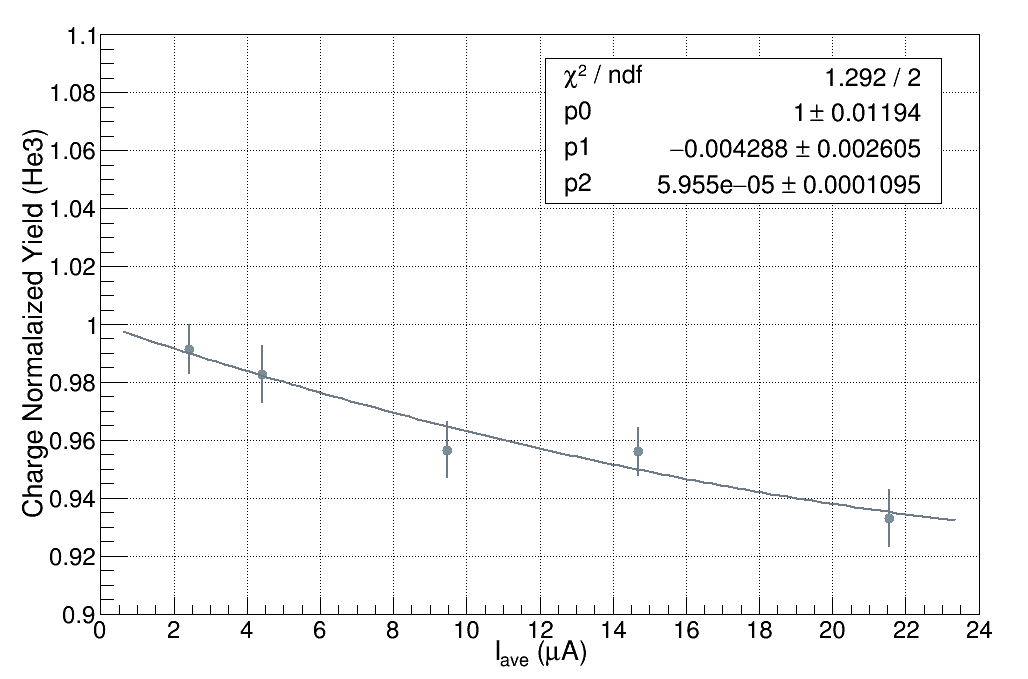
\includegraphics[width=\linewidth]{y_he3_1.png}
  \caption{Charge Normalized Yield for He3}
  \label{fig:yHe3}
\end{figure}

\section{DeuteriumTarget Boiling:} 
\begin{table}[H]
\caption{Efficiencies for H2 boiling runs}
\begin{tabular}{|>{\centering}m{0.6in} |>{\centering}m{1.3in}| >{\centering}m{1.3in}| >{\centering}m{1.3in}| >{\centering\arraybackslash}m{1.1in}|}
\hline
 \rowcolor{lightgray} Run & Cerenkov eff. (\%) & one track eff. (\%)  & trigger [T2] eff (\%)& DT (\%) \\
 \hline
919&99.98&98.724&100.3&5.625\\
918&99.99&98.62&100.5&6.97\\
920&99.98&98.37&101.2&3.81\\
921&99.98&98.08&101.6&35.21\\
923&99.98&97.58&101.1&4.076\\
\hline
\end{tabular} 
\end{table}
\begin{table}[H]
\caption{Normalized Yield and their errors for H2 runs}
\begin{tabular}{|>{\centering}m{0.3in} | >{\centering}m{0.7in}|>{\centering}m{0.7in}|>{\centering}m{0.7in}| >{\centering}m{0.7in}| >{\centering}m{1in}| >{\centering\arraybackslash}m{0.7in}|}
\hline
 \rowcolor{lightgray} Run & Current ($\mu$A) & \#good events & Total Charge ($\mu$C) &Yield & Charge Normalized Yield&  error \\
 \hline
919&2.483&96793&1325.762&234.357&0.979&0.002\\
918&4.856&115933&2737.609&229.538&0.959&0.002\\
920&9.784&52131&4902.409&222.121&0.928&0.004\\
921&14.515&48688&6936.292&217.450&0.909&0.004\\
923&21.533&52185&10334.375&213.374&0.892&0.004\\
\hline
\end{tabular} 
\end{table}
\begin{figure}[H]
  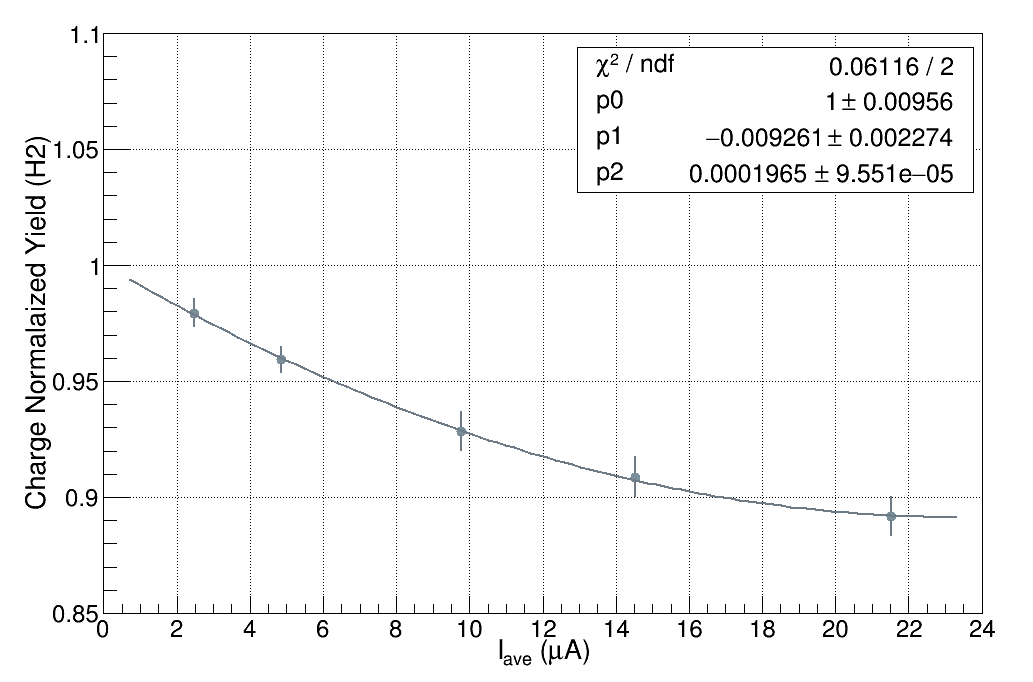
\includegraphics[width=\linewidth]{y_h2_1.png}
  \caption{Charge Normalized Yield for H2}
  \label{fig:yH2}
\end{figure}


\section{Hydrogen Target Boiling:} 
\begin{table}[H]
\caption{Efficiencies for H boiling runs}
\begin{tabular}{|>{\centering}m{0.6in} |>{\centering}m{1.3in}| >{\centering}m{1.3in}| >{\centering}m{1.3in}| >{\centering\arraybackslash}m{1.1in}|}
\hline
 \rowcolor{lightgray} Run & Cerenkov eff. (\%) & one track eff. (\%)  & trigger [T2] eff (\%)& DT (\%) \\
 \hline
901&99.9825&98.8563&100.5&3.08\\
899&99.9859&98.6726&100.8&3.41\\
897&99.9846&98.4586&100.9&3.77\\
896&99.9964&98.2092&100.1&3.68\\
895&99.987&97.8128&101.4&4.12\\
\hline
\end{tabular} 
\end{table}
\begin{table}[H]
\caption{Normalized Yield and their errors for H runs}
\begin{tabular}{|>{\centering}m{0.3in} | >{\centering}m{0.7in}|>{\centering}m{0.7in}|>{\centering}m{0.7in}| >{\centering}m{0.7in}| >{\centering}m{1in}| >{\centering\arraybackslash}m{0.7in}|}
\hline
 \rowcolor{lightgray} Run & Current ($\mu$A) & \#good events & Total Charge ($\mu$C) &Yield & Charge Normalized Yield&  error \\
 \hline
901&2.011&50379&1264.459&206.816&0.986&0.004\\
899&4.321&48705&2495.384&203.141&0.968&0.004\\
897&9.536&57093&6147.207&194.303&0.9326&0.003\\
896&13.636&54548&8928.621&193.563&0.922&0.003\\
895&20.937&105313&23805.592&186.091&0.887&0.002\\
\hline
\end{tabular} 
\end{table}
\begin{figure}[H]
  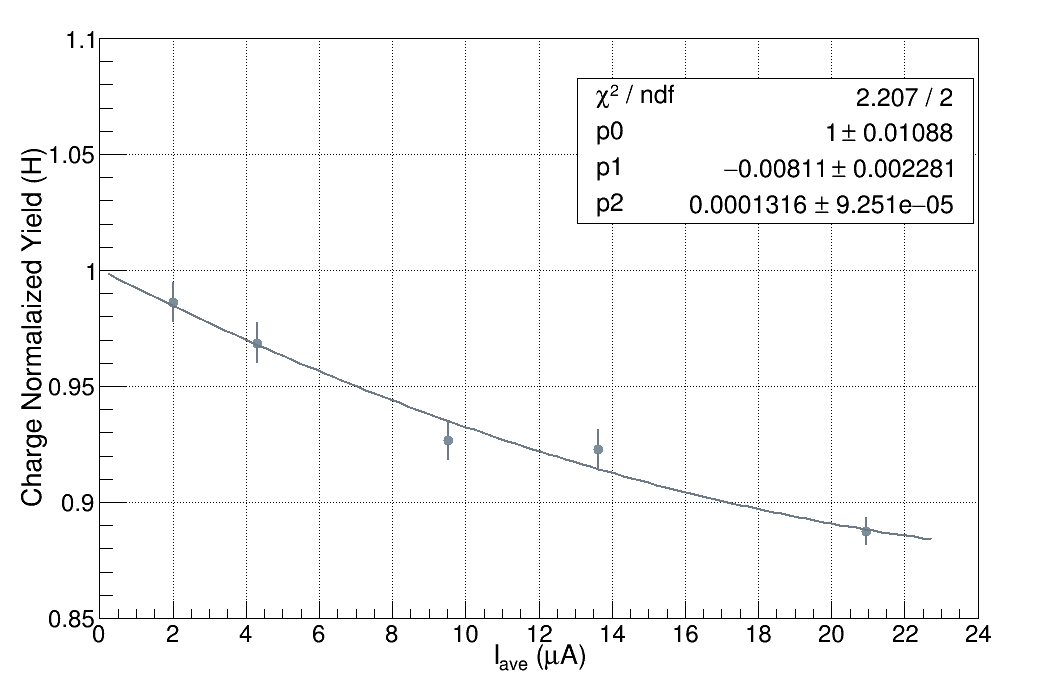
\includegraphics[width=\linewidth]{y_h_1.png}
  \caption{Charge Normalized Yield for H}
  \label{fig:yH2}
\end{figure}







\end{document}